\section{Method}
\subsection{Region Adjacency Graphs}
\frame
{
	\frametitle{Region Adjacency Graphs}
	
	\begin{figure}[p]
		\centering
		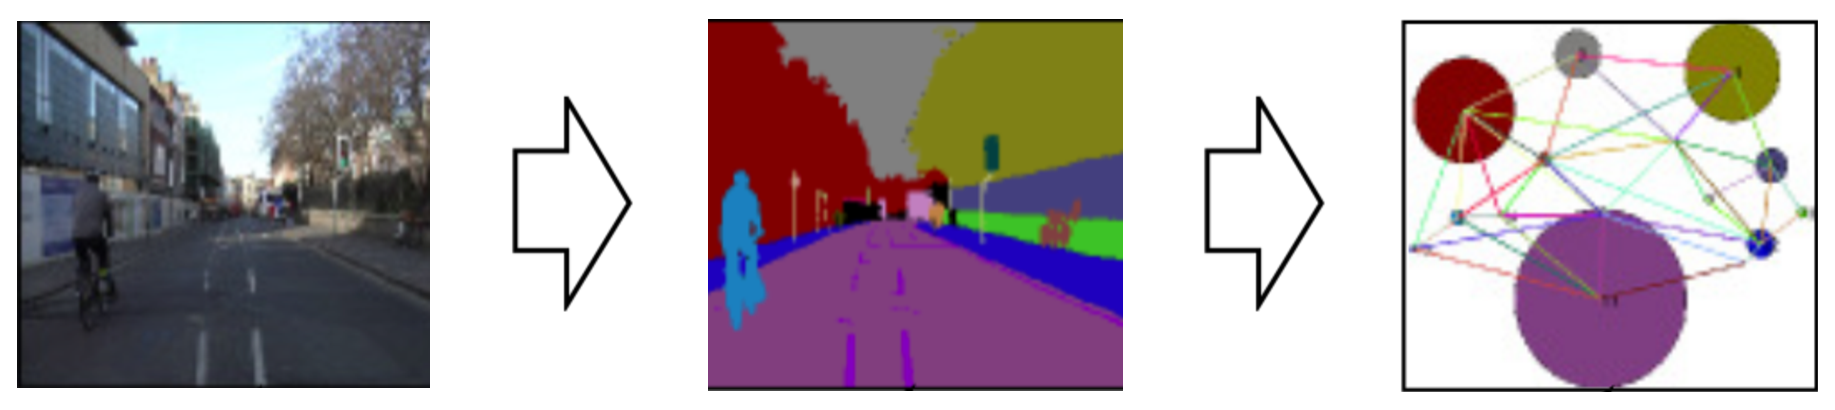
\includegraphics[width = 0.8\textwidth]{img/master/cover}
		\label{fig:rag}
	\end{figure}
	
	\begin{columns}[T]
		\column{.65\textwidth}
		\begin{itemize}
			\item Segments $\Rightarrow$ Nodes
			\item Spatial relations $\Rightarrow$ Edges
			\item Graph based segmentation method [Felzenszwalb, Huttenlocher, 2004]
		\end{itemize}
		
		
		\column{.4\textwidth}
		\vspace{-0.5cm}
		\begin{itemize}
			\item Nodes
			\begin{itemize}
				\item Color
				\item Position
				\item Size
			\end{itemize}
			\item Edges
			\begin{itemize}
				\item Mean color difference
			\end{itemize}
		\end{itemize}
	\end{columns}
	
}